\documentclass[a0paper,portrait]{baposter}
\usepackage{wrapfig}
\usepackage{lmodern}
\usepackage[utf8]{inputenc} %unicode support
\usepackage[T1]{fontenc}
\selectcolormodel{cmyk}
\graphicspath{{figures/}} % Directory in which figures are stored
\newcommand{\compresslist}{%
\setlength{\itemsep}{0pt}%
\setlength{\parskip}{1pt}%
\setlength{\parsep}{0pt}%
}
\newenvironment{boenumerate}
  {\begin{enumerate}\renewcommand\labelenumi{\textbf\theenumi.}}
  {\end{enumerate}}
\begin{document}
\definecolor{alizarin}{rgb}{0.82, 0.1, 0.26}
\definecolor{airforceblue}{rgb}{0.36, 0.54, 0.66}
\definecolor{babypink}{rgb}{0.96, 0.76, 0.76}
\definecolor{darkgreen}{cmyk}{0.8,0,0.8,0.45}
\definecolor{lightgreen}{cmyk}{0.8,0,0.8,0.25}
\definecolor{aqua}{rgb}{0.0, 1.0, 1.0}
\definecolor{amethyst}{rgb}{0.6, 0.4, 0.8}
\begin{poster}
{
grid=false,
headerborder=open, % Adds a border around the header of content boxes
colspacing=1em, % Column spacing
bgColorOne=white, % Background color for the gradient on the left side of the poster
bgColorTwo=white, % Background color for the gradient on the right side of the poster
borderColor=amethyst, % Border color
headerColorOne=babypink, % Background color for the header in the content boxes (left side)
headerColorTwo=lightgreen, % Background color for the header in the content boxes (right side)
headerFontColor=black, % Text color for the header text in the content boxes
boxColorOne=white, % Background color of the content boxes
textborder=rounded, %rectangle, % Format of the border around content boxes, can be: none, bars, coils, triangles, rectangle, rounded, roundedsmall, roundedright or faded
eyecatcher=false, % Set to false for ignoring the left logo in the title and move the title left
headerheight=0.11\textheight, % Height of the header
headershape=rounded, % Specify the rounded corner in the content box headers, can be: rectangle, small-rounded, roundedright, roundedleft or rounded
headershade=plain,
headerfont=\Large\textsf, % Large, bold and sans serif font in the headers of content boxes
%textfont={\setlength{\parindent}{1.5em}}, % Uncomment for paragraph indentation
linewidth=2pt % Width of the border lines around content boxes
}
{}
%
%------------------------------------------------------
%	TITLE AND AUTHOR NAME
%------------------------------------------------------
%
{
\textsf %Sans Serif
{{\color{red} Strengthy: A Fitness Tracking Webapp}
}
} % Poster title
%
%
{\sf\\
Dylan Bolger, Hayden Pope
\vspace{0.1em}\\
\large{Department of Computer Science\\
Missouri State University, MO, USA}}
{
\includegraphics[width=38mm]{img/Missouri_State_logo.png}}

\headerbox{Abstract}{name=introduction,column=0,row=0, span=3}{
	For thousands of years fitness and physical exercise has been apart of many
	peoples' lives. In the modern age, many people seek to utilize their
	technology in their fitness endevours. While many proprietary and closed-source
	solutions exists, there are not many self-hostable, open-source applications
	avalible.
	% Copied from outline
	Our proposal is to develop a web application to track weightlifting sessions, progress, and statistics. This web-app will allow users to create personal accounts to track their information. We will allow the user to upload their data from days at the gym and be able to watch their progress as they continue to go to the gym. It will also show useful calculations, such as percentages of your 1RM (One repetition max). Statistics like progress prediction of the user and analysis will be included. Users will also be able to create their own workout plans, or routines. The routines will suggest values in order for the user to make meaningful progression at the gym. Users can also record their weight.
}

\headerbox{Experiments}{name=info,column=2,row=0,span=1, below=introduction}{
\begin{center}
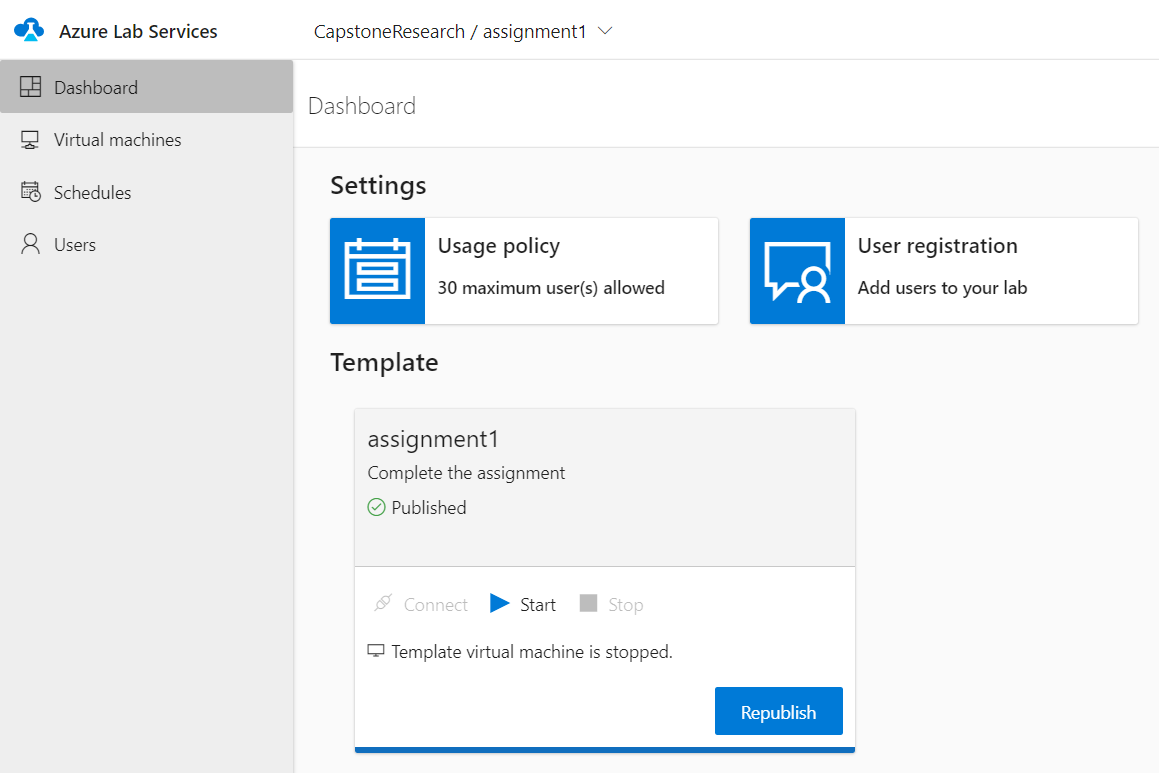
\includegraphics[width=66mm]{img/1.png}
The growth of cloud computing is growing increasingly due to its accessing convenience, unlimited amount of resources, the 24/7 IT support, and the affordable cost.
\end{center}
}

\headerbox{Motivation}{name=model,column=0,below=introduction,span=2}{
	We workout often ourselves, and were unsatisfied with the avalible options
	for fitness tracking. In addition we wanted to create an for users who
	are concerned about data privacy, and open source software. We aim to
	provide a drop-in replacement that has all the features and functionality
	of major closed-source competetors.
}

\headerbox{Proposed Solution}{name=mcs,column=0,below=model,span=2}{
\begin{itemize}
\item Step 1: Select Dashboard from the left side of the screen. Once you have selected Dashboard, look for the area labeled Marketplace and select Marketplace (Fig.1).
\item Step 2: Type in Lab Services in the search bar and press enter. Then select Lab Services (preview). After you have done that, you will select button that says Create located on the right side of the page. Once you have selected Create, you will be taken to a screen where you will  need to fill out information pertaining to the new lab service being created. Once you have filled out the information, select create.
\item Step 3: Return back to the Dashboard (as described in Step 1)  and select the name of the lab you created in Step 2 (Fig.1).
\item Step 4: Once you have selected the lab, you will be taken to the following screen. Once on that screen, you will then need to select the link titled Create a lab at  http://lab.azure.com (Fig.2).
\item Step 5: Once you have selected the link, you will be taken to a new page that will allow you to create a lab environment to begin the creation of the new lab, you will first select + New Lab. Once you have selected that, you will need to rename your lab and set the number of students you want to allow access to the lab. Once completed filling out the information, select save.
\item Step 6: Once you have selected Save, you will be taken to another page that will require you to select the size of your machine(s), the region, and the operating system. Once you have filled out the information you will select Next.
\item Step 7: Once Next has been select, you will need to enter a Username and Password for individuals to have access to your labs. Once the information has been filled out, you will need to select Create. (Do not make this username and password your own personal information because you will need to provide this information to all the individuals that will be accessing your lab.
\item Step 8: Once you have selected Create, you will now need to wait about 20 minutes for the lab to be created.
\item Step 9: Once the lab has been created, you will need to fill out some required information and select publish. Publishing will take about an hour to complete.
\item Step 10: Once the lab has been published, you will then be taken to a dashboard that allows you to control the main virtual machine. With this main virtual machine, you will be able to upload whatever information would like and it will be available on all other virtual devices for the environment you created (Fig.3).
\end{itemize}
}

\headerbox{Results}{name=screen,column=2,span=1,below=info}{ % To reduce this block to 1 column width, remove 'span=2'
%The development team used the ASP.Net Web Forms development stack to create this project. On top of the standard web technologies, the Web Forms development stack uses a Microsoft SQL Server database for data retrieval/storage, ASP Web Form Controls for front-end development and C\# for back-end development.

\begin{center}
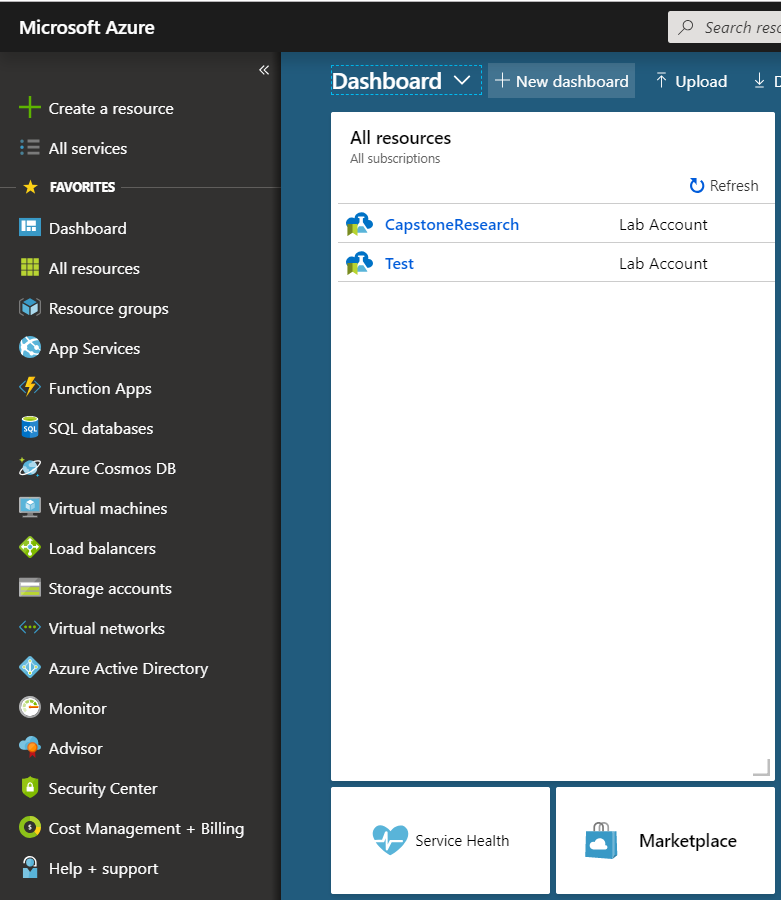
\includegraphics[width=60mm]{img/2.png}
\end{center}

%Additionally, the Bootstrap front-end library was also used for various components of the web pages to create responsive elements. Some of the associated tools that were used for development included Visual Studio Community 2016 as the main integrated development environment (IDE), Microsoft SQL Server Management Studio for database management and Azure Web Services for project deployment.
}

\headerbox{Conclusions and Future Work}{name=sea,span=3,column=0,below=mcs}{
%\includegraphics[width=151mm]{GUI1_revised.jpg}
We have come to the conclusion that LaaS is a effective and useful service that can be easily set up by any individual. After looking at the projected growth of LaaS, we have concluded that LaaS will save schools and companies a lot of money and increase the amount of individuals who use the service because of its’ convenience. We have also concluded that LaaS environments will become a popular option for universities within the next few years. We will continue our expand our knowledge on LaaS and well as learn more about the cloud and the useful services that can be provided by the cloud.
}

%\headerbox{Conclusions and Future Work}{name=conclusion,column=2,below=screen,span=1}{
%We have come to the conclusion that LaaS is a effective and useful service that can be %easily set up by any individual. After looking at the projected growth of  LaaS, we have %concluded that LaaS will save schools and companies a lot of money and increase the amount %of individuals who use the service because of its’ convenience.
%}

\end{poster}

\end{document}
